
\documentclass{sig-alternate}

\usepackage{balance}  % to better equalize the last page
\usepackage{graphics} % for EPS, load graphicx instead
\usepackage{times}    % comment if you want LaTeX's default font
\usepackage{url}      % llt: nicely formatted URLs
\usepackage{graphicx}
\usepackage{tabularx}
\usepackage{float}
\usepackage{color}
\usepackage{url}
\usepackage[noend]{algpseudocode}
\usepackage{algorithm}
\usepackage{verbatim}
\usepackage{mathtools}
\usepackage{caption}
\usepackage{subcaption}
\usepackage{minted}
\usepackage{epstopdf}
%\usepackage{amsmath}
\let\proof\relax
\let\endproof\relax
\usepackage{amsthm}
\usepackage{thmtools}
\usepackage{xspace}
\usepackage{multirow}
\usepackage[colorlinks,citecolor=blue,pdftex]{hyperref}
\usepackage{wasysym}
% \usepackage{enumitem}
\usepackage{tabularx}
\usepackage{microtype}
\usepackage{caption}
\usepackage[skip=0pt, margin=5pt]{subcaption}
\usepackage{soul}

% compress lists
% \setlist{nolistsep}

\newcommand{\note}[2]{{\color{#1} {#2}}}
\newcommand{\andrew}[1]{\note{red}{Andrew: #1}}
\newcommand{\bill}[1]{\note{red}{Bill: #1}}
\newcommand{\shrainik}[1]{\note{cyan}{Shrainik: #1}}
\newcommand{\reviewmeta}[1]{\note{black}{#1}}
\newcommand{\reviewone}[1]{\note{black}{#1}}
\newcommand{\reviewtwo}[1]{\note{black}{#1}}
\newcommand{\reviewthree}[1]{\note{black}{#1}}
\DeclareGraphicsExtensions{.pdf,.png}
\graphicspath{{./figures/}}

%\newtheorem{lemma}{Lemma}[section]
%\theoremstyle{definition}
%\newtheorem{definition}{Definition}[section]
%\newtheorem{example}{Example}[section]

\declaretheorem[numberwithin=section]{definition}

\newcommand{\ie}{{\em i.e.}\xspace}
\newcommand{\eg}{{\em e.g.}\xspace}
\newcommand{\cf}{{\em c.f.}\xspace}
\newcommand{\ea}{{\em et~al.}\xspace}
\newcommand{\aka}{{\em a.k.a.}\xspace}

%%%%%%%%%%%%%%%%%%%%%%%%%%%%%%%%%%%%%%%%%%%%%%%%%%%%%%%%%%%%%%%%%%%%%
\newcommand{\figref}[1]{\hyperref[#1]{Figure~\ref*{#1}}}
\newcommand{\secref}[1]{\hyperref[#1]{\S\ref*{#1}}}
\newcommand{\tabref}[1]{\hyperref[#1]{Table~\ref*{#1}}}
\newcommand{\defref}[1]{\hyperref[#1]{Definition~\ref*{#1}}}
\renewcommand{\eqref}[1]{\hyperref[#1]{Eq.~(\ref*{#1})}}
\newcommand{\lstref}[1]{\hyperref[#1]{Listing~\ref*{#1}}}
\newcommand{\heading}[1]{\vspace{4pt}\noindent\textbf{#1}}
\newcommand{\topheading}[1]{\noindent\textbf{#1}}
\newcommand{\noheading}[0]{\vspace{4pt}\noindent}
\newcommand{\program}[1]{\texttt{#1}}
\newcommand{\term}[1]{\texttt{#1}}
\newcommand{\captiontext}[1]{\textsf{\normalsize #1}}
%%%%%%%%%%%%%%%%%%%%%%%%%%%%%%%%%%%%%%%%%%%%%%%%%%%%%%%%%%%%%%%%%%%%%
\newcommand{\ms}{\,\text{ms}\xspace}
\newcommand{\us}{\,\text{$\mu$s}\xspace}
\newcommand{\ns}{\,\text{ns}\xspace}
%%%%%%%%%%%%%%%%%%%%%%%%%%%%%%%%%%%%%%%%%%%%%%%%%%%%%%%%%%%%%%%%%%%%%

\newcommand{\ocat}{\Omega_\textit{catalog}}
\newcommand{\ocod}{\Omega_\textit{code}}
\newcommand{\oman}{\Omega_\textit{manual}}
\newcommand{\oexe}{\Omega_\textit{execution}}

\newcommand{\socat}{\omega_\textit{catalog}}
\newcommand{\socod}{\omega_\textit{code}}
\newcommand{\soman}{\omega_\textit{manual}}
\newcommand{\soexe}{\omega_\textit{execution}}

\newcommand{\sqlshare}{SQLShare}
\newcommand{\SQLSHARE}{SQLSHARE}

\providecommand{\e}[1]{\ensuremath{\times 10^{#1}}}
\newenvironment{packed_item}{
\begin{itemize}
   \setlength{\itemsep}{1pt}
   \setlength{\parskip}{0pt}
   \setlength{\parsep}{0pt}
}
{\end{itemize}}

\newcommand\xqed[1]{%
  \leavevmode\unskip\penalty9999 \hbox{}\nobreak\hfill
  \quad\hbox{#1}}
\newcommand\marker{\xqed{$\square$}}

\newenvironment{packed_enum}{
\begin{enumerate}
   \setlength{\itemsep}{1pt}
   \setlength{\parskip}{0pt}
   \setlength{\parsep}{0pt}
}
{\end{enumerate}}

\CopyrightYear{2016} 
\setcopyright{acmcopyright}
\conferenceinfo{SIGMOD'16,}{June 26-July 01, 2016, San Francisco, CA, USA}
\isbn{978-1-4503-3531-7/16/06}\acmPrice{\$15.00}
\doi{http://dx.doi.org/10.1145/2882903.2882957}
%Authors, replace the red X's with your assigned DOI string.

\clubpenalty=10000 
\widowpenalty = 10000
\newcommand{\todo}[1]{\textcolor{red}{TODO: #1}\PackageWarning{TODO:}{#1!}}

\newcommand{\AUTHORS}{Shrainik Jain, Dominik Moritz, Daniel Halperin, Bill Howe, Ed Lazowska}
\newcommand{\TITLE}{\sqlshare: Results from a Multi-Year SQL-as-a-Service Experiment}
\newcommand{\TITLECLEAN}{\sqlshare: Results from a Multi-Year SQL-as-a-Service Experiment}
\newcommand{\KEYWORDS}{Keywords} % Used below in ACM keywords
% \newcommand{\CONFERENCE}{Under submission}


\begin{document}

\title{\TITLE}


\numberofauthors{1}
\author{
\alignauthor
 Shrainik Jain, Dominik Moritz, Daniel Halperin, Bill Howe, Ed Lazowska\\
       \affaddr{Computer Science and Engineering Department, University of Washington},
       \affaddr{Seattle, WA, USA}\\
       \email{\{shrainik, domoritz, dhalperi, billhowe, lazowska\}@cs.washington.edu}
}

\maketitle

\begin{abstract}
We analyze the workload from a multi-year deployment of a database-as-a-service platform targeting scientists and data scientists with minimal database experience.  Our hypothesis was that relatively minor changes to the way databases are delivered can increase their use in ad hoc analysis environments.  The web-based \sqlshare{} system emphasizes easy dataset-at-a-time ingest, relaxed schemas and schema inference, easy view creation and sharing, and full SQL support. We find that these features have helped attract workloads typically associated with scripts and files rather than relational databases: complex analytics, routine processing pipelines, data publishing, and collaborative analysis. Quantitatively, these workloads are characterized by shorter dataset ``lifetimes'', higher query complexity, and higher data complexity. \reviewmeta{We report on usage scenarios that suggest SQL is being used in place of scripts for one-off data analysis and ad hoc data sharing.
The workload suggests that a new class of relational systems emphasizing short-term, ad hoc analytics over engineered schemas may improve uptake of database technology in data science contexts.}
Our contributions include a system design for delivering databases into these contexts, a description of a public research query workload dataset released to advance research in analytic data systems, and an initial analysis of the workload that provides evidence of new use cases under-supported in existing systems.
\end{abstract}

\section{Introduction}
\label{sec:introduction}

We recently completed a four-year exercise to study the use of database technology in science and data science, where scripts and files are the de facto standard for data manipulation and analytics. 
Database technology has had limited uptake in these environments, in part due to the overhead in designing a schema and setting up a permanent database infrastructure.  Changing data and changing requirements make it difficult to amortize these upfront costs, and as a result analysts tend to retreat to manipulating files with scripts in R, Python and MATLAB.
Simultaneously, there is no appropriate corpus available for researchers to use to study this problem effectively.  Industry partners do not retain or do not share query workloads, and certainly do not provide public access to data. Query workloads that do exist are associate with conventional pre-engineered database applications rather than oriented toward ad hoc analysis of ad hoc datasets.

Our hypothesis was that a relatively minor set of changes to how \emph{existing} database technology is \emph{packaged and delivered} would be sufficient to convince science and data science users to adopt SQL in their day-to-day data manipulation and analysis tasks, \reviewmeta{potentially} displacing script-and-file based approaches.  To test this hypothesis, we built 
\sqlshare{}, a web-based system designed to make database technology easier to use for ad hoc tasks.  We then deployed the system as a service and logged a multi-year query log as a research corpus for further analysis.  This paper represents the release of the corpus to the database community, a description of the system that collected it, and an initial analysis of the data it contains. \reviewmeta{We also performed some informal ad-hoc interviews with our active user base, which is mostly comprised of \emph{researchers and scientists}, and some of the results and conclusions drawn are influenced by our familiarity with these users.}. 

Our ultimate goal is to design new systems to better support ad hoc data management and analytics.
Although we target researchers in the physical, life, and social sciences, we find that the requirements in data-intensive science and data-intensive business have begun to converge. The data scientists that are in high demand
share characteristics with academic researchers: a stronger math background and deep domain knowledge, 
traits that sometimes come at the expense of software and systems expertise.
In response, we designed \sqlshare{} \cite{howe2013sqlshare,howe2011database} to reduce the use of a database to a minimal workflow of just uploading data, writing queries, and sharing the results --- we attempt to automate or eliminate steps for installation, deployment, schema design, physical tuning, and data dissemination.  
We deployed this system to determine its efficacy in attracting science users and understand their requirements.  This experiment was not a controlled user study; rather, we deployed \sqlshare{} as a production service --- an ``instrument'' to collect measurements on the kind of datasets used in practice, the kinds of queries these scientists and data scientists would write, and how the specific \sqlshare{} features would be used.

In this paper, we describe the corpus we collected during this experiment, describe the \sqlshare{} system used to collect the corpus, and present findings from an initial analysis of the corpus. 
Our results show that the specific features of \sqlshare{} are associated with specific usage patterns observed in the workload dataset, and that these patterns \reviewmeta{may motivate new kinds of data systems.}
We have made the query log dataset available to the research community to inform research on database interfaces, new languages, workload optimization, query recommendation, domain-specific data systems, and visualization.  Our dataset is one of the only two known real-world SQL workloads publicly available to the database research community (the other being the Sloan Digital Sky Survey workloads~\cite{kent1994sloan}), and the only one containing primarily ad hoc, hand-written queries over user-uploaded datasets.

\reviewmeta{The workload suggests that some of our users are comfortable expressing complex tasks in SQL (binning, integration across many tens of datasets) and making use of advanced language features such as window functions.
Further, there is evidence that by relaxing schema requirements and inferring structure automatically, we allow analysts to use SQL itself to incrementally impose structure by writing views: assigning types, renaming columns, cleaning bad values, reorganizing tables --- tasks normally associated with offline preprocessing in a general purpose language.}

Although SQL itself appears useful in this context, support for complex query authoring emerges as an important research topic:
query recommendation, editors, debuggers, new languages supporting the common idioms found in this workload all appear well-motivated. \reviewmeta{SQL has enjoyed a resurgence as an important interface for analytics without necessarily relying on engineered schemas (e.g., HIVE \cite{hivesql}, SparkSQL \cite{armbrust2015spark}, and Schema-free SQL \cite{schemafreesql}). More recently Metanautix \cite{metanautix} has adopted SQL for image and video processing tasks. 
Our work provides further evidence of SQL's utility in non-traditional contexts, especially in science.}

We find that conventional database views are remarkably useful for a variety of tasks in science and analytics environments: protected data sharing, workflow provenance, data publishing, abstraction for data processing pipelines.  To encourage the use of views, we made view creation a side effect of query authoring and were careful to erase any distinction between physical tables and virtual views --- both views and tables were considered a ``dataset.''

Sharing results with collaborators without emailing scripts and files emerged as an important use case.  Collaborators reported browsing long chains of nested views to understand the provenance of a dataset.  Snippets from one query were reused in other queries routinely.  Shared datasets could be queried and manipulated without requiring data to be downloaded first.  Altogether, these features led to workloads that involved very short data lifetimes: Data could be brought into the database easily, analyzed briefly with SQL, and shared with other partners with a click.  The users report that these short-lifetime workloads were typically implemented as scripts in R or Python; \sqlshare{} demonstrates that they can be supported in the database itself with minimal system changes.

We intend the database community to use this paper as a reference for understanding how non-experts use SQL ``in the trenches,'' as a description of a workload dataset to drive further research, and as a baseline for comparison with new database systems targeting similar users.
This paper makes the following contributions:

\begin{itemize}
\itemsep0em
\item A new publicly available ad hoc SQL workload dataset of $24275$ hand-written queries over $3891$ user-uploaded tables provided by scientists and data scientists in the life, physical, and social sciences.
\item A description of the important features of the \sqlshare{}, a system designed to increase uptake of database technology for ad hoc analysis and deployed as the instrument used to collect the workload.
\item An initial analysis of the \sqlshare{} workload linking the features of \sqlshare{} to specific usage patterns typically associated with scripts-and-files, along with a general characterization of these usage patterns.
\item A comparison of the \sqlshare{} workload with that of a conventional schema-first science database to provide evidence that the characteristics we uncover are unique to the \sqlshare{} experiment.
\end{itemize}

\begin{figure}[t]
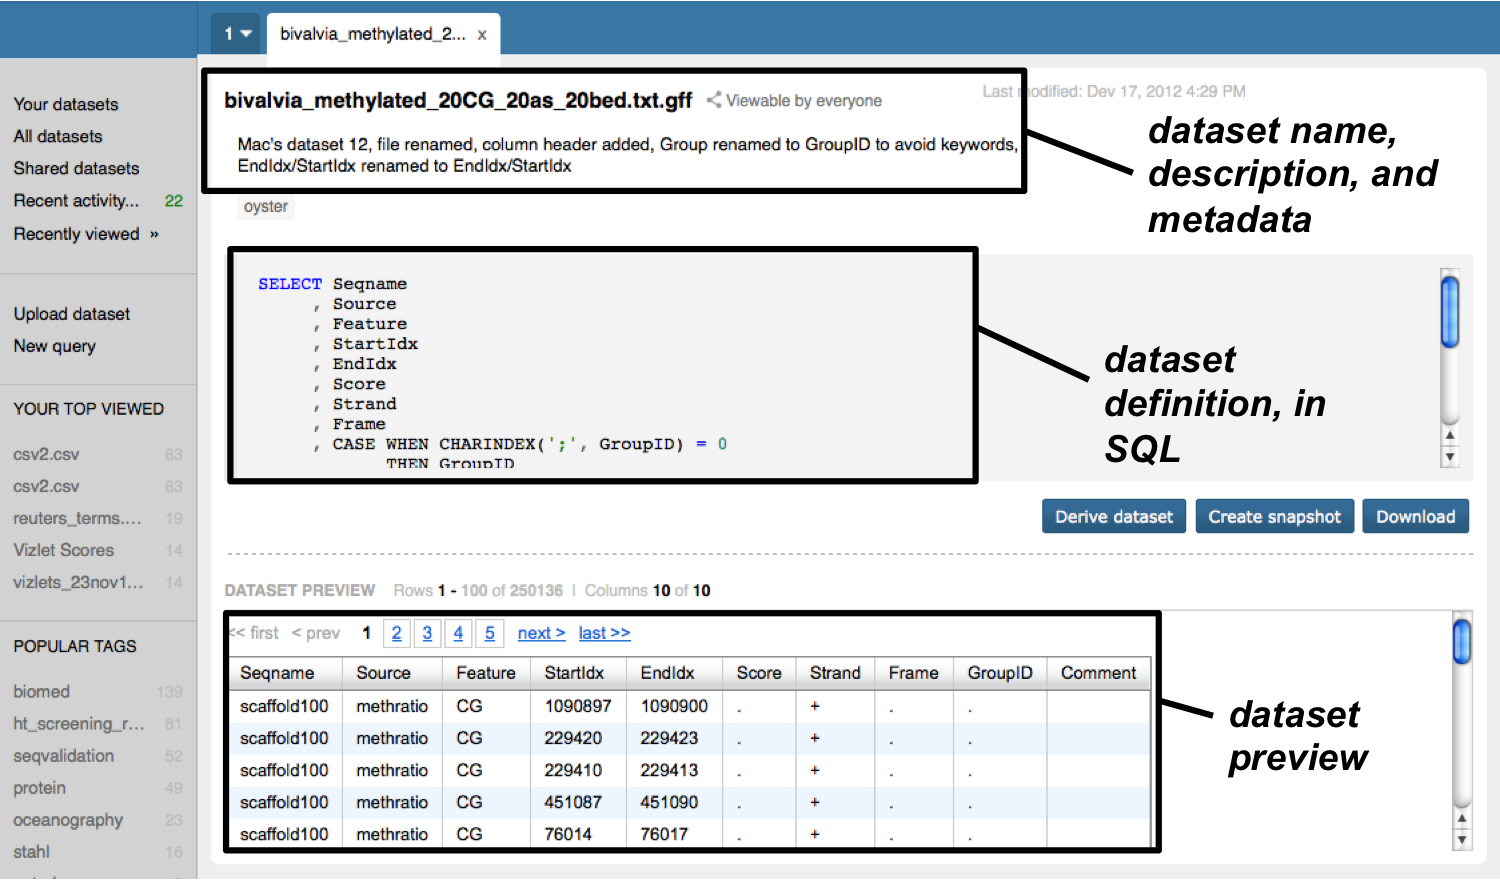
\includegraphics[width=\linewidth]{sqlshare_screenshot.png}
\caption{Screenshot of the \sqlshare{} user interface. Each dataset is a view associated with some descriptive metadata and a preview. Creating and sharing views is the primary workflow in using the system.}
\label{fig:screenshot}
\end{figure}


\section{Problem Context}
Relational databases remain underused in science (and data science) despite a natural
fit between hypothesis testing and interactive query.
Some ascribe this underuse to a mismatch between the requirements of
scientific data analysis and the models and languages of relational database systems~\cite{stonebraker:09}.
Our experience is that rows-and-columns datasets remain ubiquitous
in science, and that standard relational models and languages
remain a good conceptual fit.
We find that the key barriers to adoption lie elsewhere:

\begin{itemize}
\itemsep0em
\item 
Although collections of records are
generally appropriate, datasets in practice are \emph{weakly structured}: 
they exhibit inconsistent types, missing and incorrect values, inconsistencies across 
column and table names, horizontal and vertical decomposition of logical 
datasets into sets of files. General purpose languages and collections of
files are perceived to be the highest level of abstraction that can accommodate
this heterogeneity.

\item Daily activity results in long chains of \emph{derived datasets}.  Raw data are cleaned,
restructured, integrated, processed, and analyzed --- each step in the chain results in 
a derived dataset.  The processing history of the dataset is important for provenance
purposes.  These derived datasets may be virtual or materialized, but in either case
ease of recomputation is considered paramount.  The natural inclination is to model
the processing pipeline as a sequence of scripts, giving rise to workflow management
systems designed to manage the execution and sharing of script-based processing~\cite{cohen2011search,pegasus,ogasawara2011algebraic,escienceworkflow}.
\item As workloads become increasingly analytical, declarative languages are perceived
to be increasingly limited.  The emergence of impoverished SQL languages that lack support
for standard features exacerbates the problem.\footnote{For example, the popular HIVE SQL dialect
only supports subqueries in the FROM clause and does not support window functions, complicating 
common analytical idioms that are naturally expressed in GPLs using loops.}
\item Inter-institution collaboration demands
selective \emph{sharing} of data, analysis steps, and results on-demand.
\item Teams of researchers exhibit significant \emph{diversity}, with varying backgrounds, 
varying experience levels, and varying tolerance for technical barriers.  
Data systems that require significant installation, configuration,
and loading steps before delivering value are perceived as ``maybe good for database experts, 
but not right for me.''
\item Highly dynamic analysis environments result in \emph{short data lifetimes}: datasets are presented to the system, analyzed, and then put aside. In contrast, conventional database applications tend to emphasize 
a permament, pre-engineered schema. The transient nature of data makes it difficult to amortize the cost of schema design and data loading in a conventional database and motivate a tighter interaction loop for incorporating new data sources.
\end{itemize}

Given these requirements, there is a temptation to design a new system from scratch targeting these requirements. Instead, we consider the null hypothesis: that existing database systems are largely equipped to support these new environments, provided we change their interfaces to support these new workflows.  We consider how to change the ``delivery vector'' of relational databases by emphasizing certain features (full SQL, views) and de-emphasizing or automating the use of other features (fixed, pre-engineered schemas).

In this paper, we first formalize these requirement and show how we address them in \sqlshare{}. Next we analyze \sqlshare{} workload to show how we fared on fulfilling these requirements over the last 4 years. 
We then look at a comparison of \sqlshare{} workload with the SDSS workload and show how \sqlshare{} queries are more diverse and very complex. 
We conclude with a discussion about the non-traditional workflows generated over \sqlshare{}. We show that by making use of databases simpler, \sqlshare{} enabled novice database users to build data analytic skills and focus on science and domain expertise.

\section{\SQLSHARE{} Platform Features}
\label{sec:sqlshare}

The \sqlshare{} \cite{howe2011database} platform was designed, built and deployed to deliver database technology into science contexts, and, as a side effect, collect a workload dataset for use by the database research community. 
\tabref{t:notation} summarizes the key features required to support science and data science use cases. Next we look at how each of these feature were built into \sqlshare.

\begin{table}
\begin{small}
\caption{Summary of observed requirements in science and data science environments.}
\label{t:notation}
\centering
\begin{tabular}{|p{0.3\linewidth}|p{0.23\linewidth}|p{0.33\linewidth}|}\hline
Requirement & Feature & Evidence \\
\hline
Weakly structured data & Relaxed schemas & Casting, cleaning, integration \\ \hline
Derived datasets & First-class views & Deep view chains, reuse, abstraction \\ \hline
Collaborative sharing & User-controlled permissions & Public datasets, fine-grained sharing \\ \hline
Complex manipulation & Full SQL & Use of complex idioms and features \\ \hline
Diverse users & SaaS & Broad use \\ \hline
Low data lifetime & Relaxed schemas & ``One-pass'' workloads\\ \hline
\end{tabular}
\end{small}
\end{table}

\sqlshare{} is a cloud-hosted data management system for science emphasizing relaxed schemas and collaborative analysis.
By ``relaxed schemas,'' we mean that data can be uploaded as is, and column types are inferred automatically from the data upon ingest rather than prescribed by users.
Moreover, the interfaces are designed to accommodate the management of hundreds or
thousands of datasets per user instead of a single fixed schema linked by integrity constraints.  \sqlshare{} supports a ``Sea of Tables'' model rather than a pre-engineered schema.
In this sense, it supports usage patterns like those of a filesystem rather than a database: Datasets can be freely created without regard to global constraints. Each dataset is a collection of typed records and has a name, but otherwise the system makes no assumptions.

\sqlshare{} supports exploratory analysis by emphasizing the derivation and
sharing of virtual datasets via relational views, and eschews destructive update at the tuple
level in favor of dataset-level versioning.  Tasks typically considered out of scope for relational databases,
including preliminary data cleaning, timeseries analysis, and statistical analysis, are implemented by creating multiple layers of views.
For example, nutrient information in an environmental sensing application may contain string-valued flags indicating missing numeric data,
incorrect column names, and may comprise many separate files instead of one logical dataset.
Instead of demanding that these issues be resolved prior to ingest into the system, \sqlshare{} encourages data to
be uploaded ``as-is'' and repaired using database features.  Users
may write one view  to rename columns, another to replace missing values cast types,
a third to integrate the files into one logical dataset, and a fourth to bin the data by time
to compute an hourly average.  Any of these views can be shared with collaborators as needed, and
complete provenance of how the final result was constructed from raw data is available for inspection.

\sqlshare{} was deployed and managed as a cloud-hosted service, which has been critical to the success of the experiment: The
backend system was developed and supported by either zero or one developer at any time, thanks to the automatic failure handling and simplified deployment offered by the cloud providers.

The \sqlshare{} experiment has been running in various forms since 2011, and we have attracted hundreds of science users who have run tens of thousands of queries over thousands of datasets.

\subsection{Relaxed Schemas} 
Datasets are uploaded to \sqlshare{} via the REST interface. Although we anticipated adding support for a number of different file formats, in practice we found that nearly all data was presented in some variant of row-delimited and field-delimited format, e.g. csv. Files are staged server-side and briefly analyzed to infer column types and assign default column names if necessary.  Somewhat surprisingly, almost 50\% of the datasets uploaded did not have column names supplied in the source file. 
\begin{figure}[h]
\centering
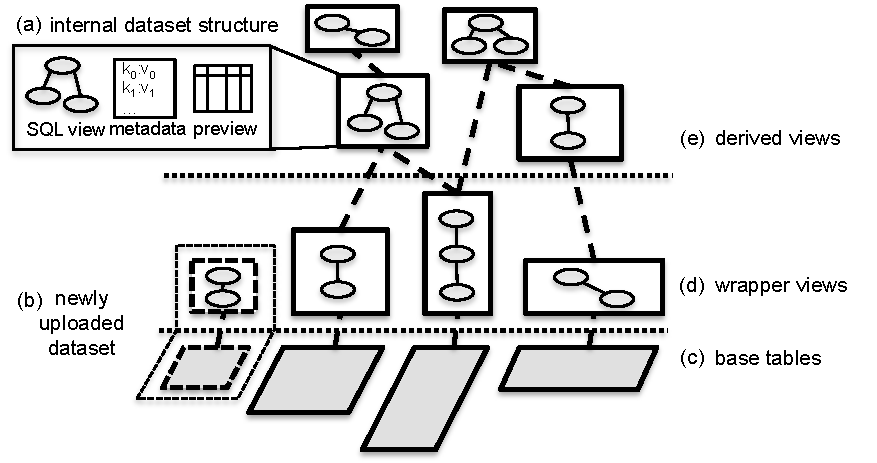
\includegraphics[width=0.9\columnwidth]{datamodel.pdf}
\caption{The \sqlshare{} data model. (a) The internal structure of a dataset, consisting of a relational view, attached metadata, and a cached preview of the results. (b) A newly uploaded datasets creates both a physical base table and an initial (trivial) wrapper view. (c) The physical data are stored in base tables, but never modified directly. (d) Wrapper views are indistinguishable from other \sqlshare{} datasets, except that they reference physical base tables. (e) Derived datasets can be created by any user. Permissions are managed in the underlying database.}
\label{fig:datamodel}
\end{figure}
Once a schema is derived, the appropriate table is created in the database and the file is ingested.  By staging the file server-side we ensure robustness: if ingest fails, we can retry without forcing the user to re-upload the data.  To infer the format, we consider various row and column delimiter values until the first $N$ rows can be parsed with identical column counts.  To infer column types, the first $N$ records are inspected. 
For each column, the most-specific type is identified.  For example, if every value can be successfully cast as an integer, the type is assumed to be an integer.  This prefix inspection heuristic can fail, and non-integer types may be encountered further down in the dataset.  
In that case, the database raises an exception, we revert the type to a string via ALTER TABLE, and the ingest continues.  
Besides mixed-type columns, we also tolerate non-uniform row lengths. Additional columns are created as needed to accommodate the longest row, and these columns are padded with NULL for rows that do not supply appropriate values. A total of 9\% of the datasets uploaded to \sqlshare{} made use of this feature. 

\reviewthree{Our goal with this data ingest process is to tolerate (and ideally to flag and expose) many types of data problems, including problems with the structure, types, or values.  We have designed the system to ensure that we do not reject such dirty data, because many of our target users (\reviewmeta{researchers in physical, life and social sciences}) have no capacity to clean, reformat, or restructure the data offline. If we force them to use scripts (or even spreadsheets) to clean the data as a preprocessing step, we are essentially asserting that \sqlshare{} is irrelevant for their day-to-day tasks. Instead, we want to tolerate malformed data and encourage the use of SQL itself to scale and automate cleaning and restructuring tasks.}

\subsection{Data Model: Unifying Views and Tables}
\label{sec:datamodel}
We illustrate the data model of \sqlshare{} in \figref{fig:datamodel}. 

Views are a first-class citizen in \sqlshare{}.  Views are created in the UI (or programmatically in the REST interface) by saving a query and giving it a name.  Everything in \sqlshare{} is accomplished by writing and sharing views: Users can clean data, assess quality, standardize units, integrate data from multiple sources, attach metadata, protect sensitive data, and publish results.  We avoid forcing the user to use the CREATE VIEW syntax of the SQL standard, for two reasons: First, we want a view to be conceptually identical to a physical table --- our design principle is ``everything is a dataset.''  Second, the syntax proved awkward in initial tests with users.  

All datasets are considered read-only; the only way to modify a dataset is by changing its view definition. Using UNION queries, a view definition can be extended with new data to simulate batch INSERTs.  The advantage of this design is that provenance is maintained: an uploaded batch of data can be ``uninserted'' at a later date, and the substructure of the dataset as a sequence of batch inserts can be inspected and reasoned about.  The disadvantage of this approach is that it prevents tuple-at-a-time updates and inserts.  However, we find that a key characteristic of our target workloads is dataset-at-a-time processing, and we have not seen this design principle reported as a weakness.  The REST interface provides some convenience features for appending batches of tuples: An \texttt{append} call accepts an existing dataset name $E$ and a newly uploaded dataset name $N$ as input, and, if the schemas are compatible, the query definition associated with $E$ will be rewritten as $(E) UNION (N)$.  Downstream views and queries will automatically see the new data with no changes required.  For some applications, it is important that the data doesn't change without the consumers' knowledge.  \reviewone{In these cases, the user can \texttt{materialize} the dataset to create a snapshot that is distinct from the original view definition. \sqlshare{} does not automatically materialize views to improve performance; there is an application-specific tradeoff with freshness that we have not yet explored how to optimize.  We are exploring certain ``safe'' scenarios where we can make materialization decisions unilaterally.}

Each \emph{dataset} in \sqlshare{} is a 3-tuple ($sql$, $metadata$, $preview$), where $sql$ is a SQL query, $metadata$ consists of a short name, a long description, and a set of tags, and $preview$ is the first 100 rows of the dataset.
When a user uploads a table to \sqlshare{}, a \emph{base table} \texttt{T} is created, along with a trivial \emph{wrapper} query of the form \texttt{SELECT * FROM T}.  This design helps unify the concept of tables and views and also provides an initial example query for novice SQL users to operate from. We find in practice that editing a simple query into an ``adjacent'' query is very easy for anyone in practice; only writing a complex query from scratch is difficult.
The owner of the dataset is the user who created it; ownership cannot be transferred. Each dataset is associated with a set of keyword $tags$ to ease search and organization in the UI. The set of $permissions$ provides user-specific access. Users are not allowed to run DDL statements like \texttt{CREATE TABLE} etc. since that would make it difficult to automatically make a view on top of every table. \reviewone{Users can make a dataset public, share it with specific users, or keep it private. When sharing derived views, complex situations can arise.  The semantics for determining access to a shared resource uses the concept of \emph{ownership chains}, following the semantics of Microsoft SQL Server.  If user $A$ owns a table $T$, they can share a derived view $V_1(T)$ with user $B$ even if the table $T$ has not been shared, and user $B$ will have access.  But if user $B$ then creates a derived $V_2(V_1(T))$ and shares it with user $C$, user $C$ will encounter an error because the ownership chain $V2\rightarrow V1 \rightarrow T$ is broken (i.e., it involves two different users, $A$ and $B$.)  We are exploring whether these semantics are too conservative for our requirements, given that sharing is a first-class concept.}

\subsection{Query Processing}
Queries are submitted to \sqlshare{} primarily via the WebUI or sometimes directly through the REST API. REST server receives the query request, and assigns an identifier to the request which is sent back to the requesting client. The WebUI uses this identifier to regularly get results or check for query status. 
This was an obvious choice over an atomic request for queries as long running queries would reduce the requests the REST server can handle.
The REST server uses the MS SQL Azure's \texttt{C\#} library to run queries internally. As of now, we do not create any automatic indices, however this is a feature we might build later.
Since the dataset updates are allowed only via creation of newer datasets, we can assume that the result of query wouldn't change over time. 
This allows us to save the preview results for each dataset and serve them instead of running the query every time the dataset is accessed. However the query needs to be actually run if the user submits a `download results' request. 

\begin{figure}[t]
\centering
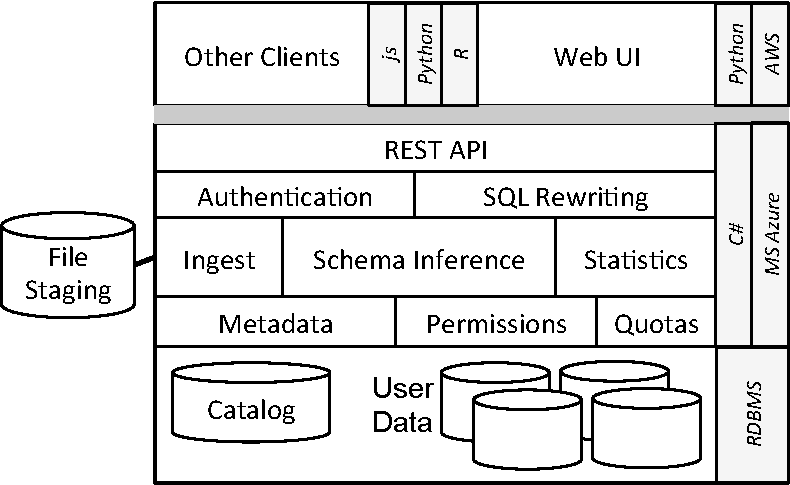
\includegraphics[width=\linewidth]{architecture.pdf}
\caption{\sqlshare{} architecture, primary user interface is the Web UI which communicates with the REST layer for dataset ingest, modification (via views) and querying. REST server interacts with the backend database which also keeps a catalog of user queries.}
\label{fig:architecture}
\end{figure}

\subsection{Architecture}
The architecture of \sqlshare{} appears in Figure \figref{fig:architecture}. The core system consists of a REST interface in front of a database system that implements the data model, query log, ingest semantics, manages long-running queries, handles exceptions, and manages authentication. The \sqlshare{} REST interface is compatible with any relational database, but it was originally deployed using the Microsoft Azure Database (originally SQL Azure). The Microsoft Azure Database is mostly interface compatible with Microsoft SQL Server, except that it requires all tables to be associated with  clustered index.  In \sqlshare{}, we avoid exposing DDL to users and therefore create a clustered index by default on all columns in the database, in column order.   
The front-end UI is in no way a privileged application; it operates the REST interface like any other client.  Indeed, other clients exist, in some cases built by the community.  For example, the R client for \sqlshare{} was written by a user based on their own requirements, and multiple javascript-based visualization interfaces have been developed. 

\subsection{Full SQL}
\reviewmeta{We built \sqlshare{} in part to faciliate access to the features of the full SQL standard, finding from our experience working with scientists that their use cases frequently required features that are not provided by simplified SQL dialects such as those found in HIVE~\cite{hivesql} or Google Fusion Tables~\cite{gonzalez2010google}.
Specifically, window functions, unrestricted subqueries, rich support for dates and times, and set operations all appeared necessary in early requirements analysis. Since the interface is organized around a workflow of copying and pasting snippets of SQL from existing queries (a practice that in some cases may even be beneficial \cite{cloneuse} \cite{kim2005empirical}), we see evidence of users writing increasingly complex queries over time.

To support full SQL, we parse each query using a third-party standards-compliant SQL grammar in ANTLR, which we modified to accommodate details of the SQL Azure database and avoid common user pitfalls.  For example, when creating a view, we automatically remove any ORDER BY clause to comply with the SQL standard.

\figref{fig:screenshot} shows a screenshot of the SQL editor.  Users edit queries directly in the browser, but can access recently viewed queries to copy and paste snippets as needed.} We analyze the usage of SQL features in Section \ref{sec:fullsql}.


\section{Overview of the \SQLSHARE{}\\Workload}
\sqlshare{} logs all executed queries; this log was collected to inform research on new database systems supporting ad hoc analytics over weakly structured data.  With permission from the users, we are releasing this dataset publicly for use by the database research community.
To our knowledge, no other workload in the literature provides user-written SQL queries over user-uploaded datasets.

The \sqlshare{} workload has a total of $24275$ queries on $7958$ datasets (including $4535$ derived datasets implemented as views), authored by $591$ users over period of four years. \reviewmeta{Out of $591$ users, $260$ are from universities (indicated by a .edu address). In addition, we have interviewed a number of our top users and are familiar with their science and their requirements.} There are a total of $3891$ tables with an average of $12$ queries per table. 
\figref{fig:queriespertable} shows a histogram depicting the distribution of queries per table. Most tables are either accessed just once or they are queried $>=5$ times.

The \sqlshare{} system is not intended for large datasets; the total volume of data presently in the system is $143.02$ GB. However, users delete datasets regularly so this number doesn't represent the size of all the datasets that have ever been present \sqlshare{}.  Indeed, \reviewmeta{based on our interactions with some users, they claimed to} have developed a daily workflow of uploading data, processing it in SQL, downloading the results, and then deleting everything. 
Diversity rather than scale is the salient feature of the workload.

\reviewmeta{A short survey sent to all users to assess the effectiveness of \sqlshare{} revealed that only $6$ (out the $33$ users who responded) felt that some other off-the-shelf database system could meet their data management needs. $18$ of $33$ reported that \emph{no} other tool would work for their requirements. The remaining $9$ users mentioned that non-database tools such as iPython notebooks might be appropriate for their tasks. $23$ of $33$ users mentioned that ``\emph{ease of data upload \& cleaning}'' and ``\emph{ability to share}'' was the reason they found \sqlshare{} most helpful.}

\begin{figure}[h]
\centering
\includegraphics[width=\columnwidth]{plot_queries_per_table.eps}
\caption{Distribution of queries per table. a) About a third of the tables accessed just once. b) Greater than a third of the tables are accessed many times, with the most common table being queried 766 times, suggesting two distinct use cases.}
\label{fig:queriespertable}
\end{figure}

\paragraph{Extracting information from query logs}
\label{sec:extract}
To analyze the complexity and diversity of the \sqlshare{} logs (Section \ref{sec:workload}), we developed a framework for extracting metrics from each query and its associated plan. The metrics of importance are query length, runtime, number \& type of physical \& logical operators, number \& type of expression operators, tables \& columns referenced and operator costs. We will use these metrics to drive the discussion the later sections.

The algorithm for extraction has 2 phases. In phase 1 each query in the \sqlshare{} logs were sent to SQLServer, which returned the execution plan along with estimated result sizes and runtimes for each operator.
The format of the execution plan is XML and is obtained by setting the \texttt{SHOWPLAN\_XML} property\footnote{\url{http://msdn.microsoft.com/en-us/library/ms187757.aspx}}.
The operator tree along with interesting properties needed for further analysis is extracted from the XML document with XPath~\cite{clark1999xml}.
These properties are estimated runtimes, estimated result sizes and predicates or other properties of an operator.
Predicates for selections are split into clauses such that if one selection has a superset of predicates, it is more selective and filters out more tuples.
Expressions are also extracted via XPath.
Phase 1 extracts these properties and makes a simpler JSON plan for easier future consumption and saves it as an additional column in the query log. \figref{fig:method_phase1} provides a conceptual visualization of Phase 1.

\begin{table}[h]
\begin{subtable}{0.45\columnwidth}
\vspace{-10pt}
\centering
\vspace{-10pt}
\begin{tabular}{| p{1.2cm} | l |}
\hline
Users & $591$ \\ \hline
Tables & $3891$  \\ \hline
Columns & $73070$  \\ \hline
Views & $7958$  \\ \hline
Non-trivial Views & $4535$  \\ \hline
Queries & $24275$  \\ \hline
\end{tabular}
% \vspace{-10pt}
\caption{Workload Metadata}
\label{t:summarymetrics1}
\end{subtable}
\vspace{-10pt}
\begin{subtable}{0.45\columnwidth}
\centering
\begin{tabular}{| p{1.8cm} | l |}
\hline
Feature & Mean Value \\ \hline
Length  & $217.32$ char.  \\ \hline
Runtime & $3175.38$ s.  \\ \hline
\# of Operators & $18.12$  \\ \hline
\# of Distinct Operators & $2.71$  \\ \hline
\# of Tables accessed & $2.31$ \\ \hline
\# of Columns accessed & $16.22$ \\ \hline
\end{tabular}
% \vspace{-10pt}
\caption{Query Metadata}
\label{t:summarymetrics2}
\end{subtable}
% \vspace{-3pt}
\caption{Aggregate summary of \sqlshare{} metadata. \reviewmeta{\sqlshare{} workload has an average $12$ queries per table.}}
\end{table}

Phase 2 of the algorithm goes over each query and corresponding JSON plan and extracts other important query metadata like referenced tables, columns and views per query. This metadata is aggregated into separate tables in the query catalog for further analysis of the workload. \figref{fig:method_phase2} shows a flowchart for this phase of the algorithm.

\begin{figure*}
  \centering
  \subcaptionbox{
  Phase 1 of extracting information from query log. For each query, backend SQL Server is asked to explain it and return the corresponding XML plan. The XML is then cleaned for easier parsing and the extracted information is converted to a JSON plan for easier consumption by further steps. This JSON plan is saved back to query catalog as a new column.
  \label{fig:method_phase1}}
    {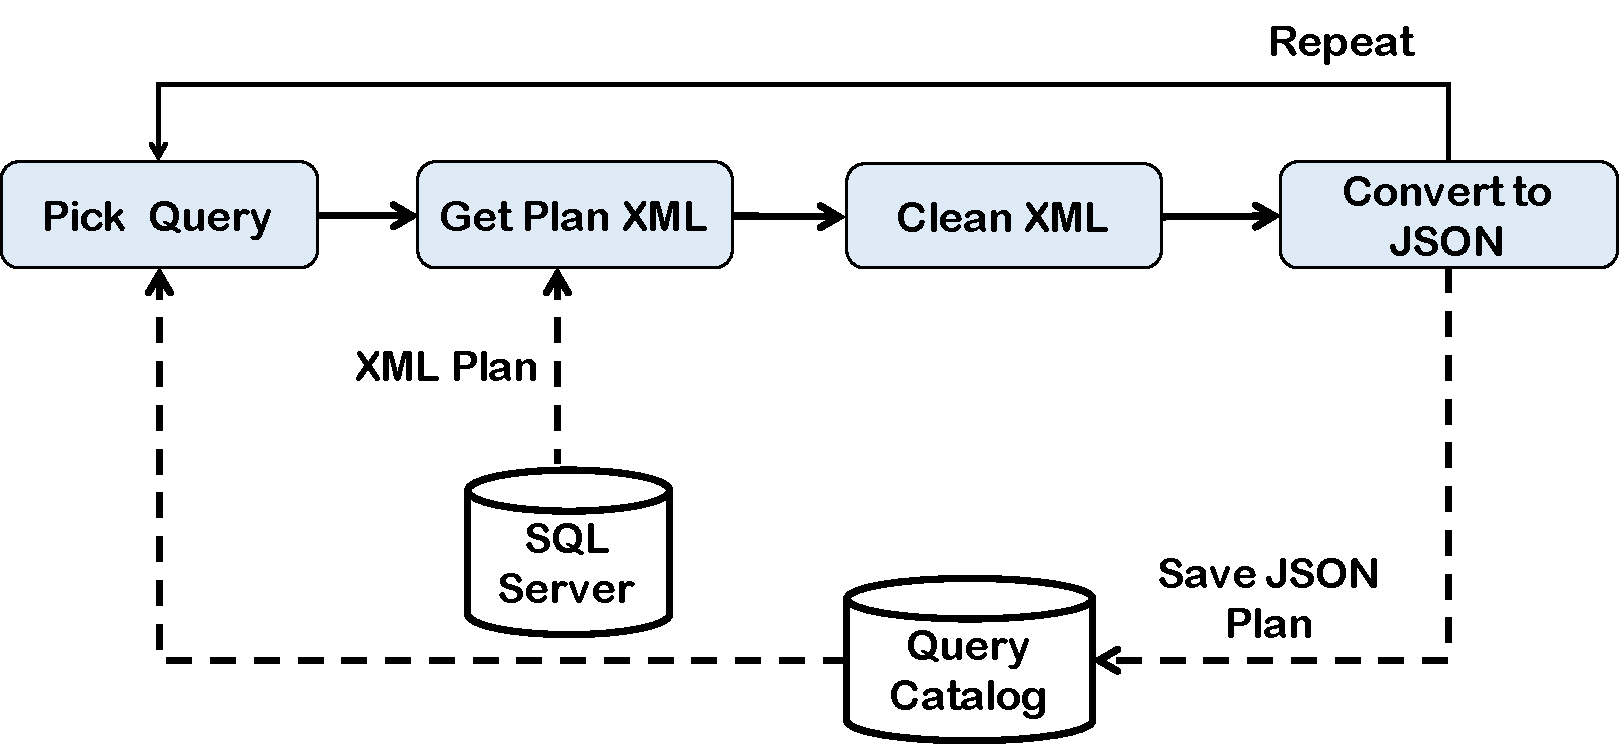
\includegraphics[width=.4\linewidth]{method_phase1.pdf}}
  \subcaptionbox{
  Phase 2 of extraction methodology picks a JSON plan from previous step. From the JSON plan, the referenced tables, columns and views are extracted and saved in separate tables in the query catalog. Next the operators, expressions and corresponding costs are extracted and saved into separate tables in the catalog as well.
  \label{fig:method_phase2}}
    {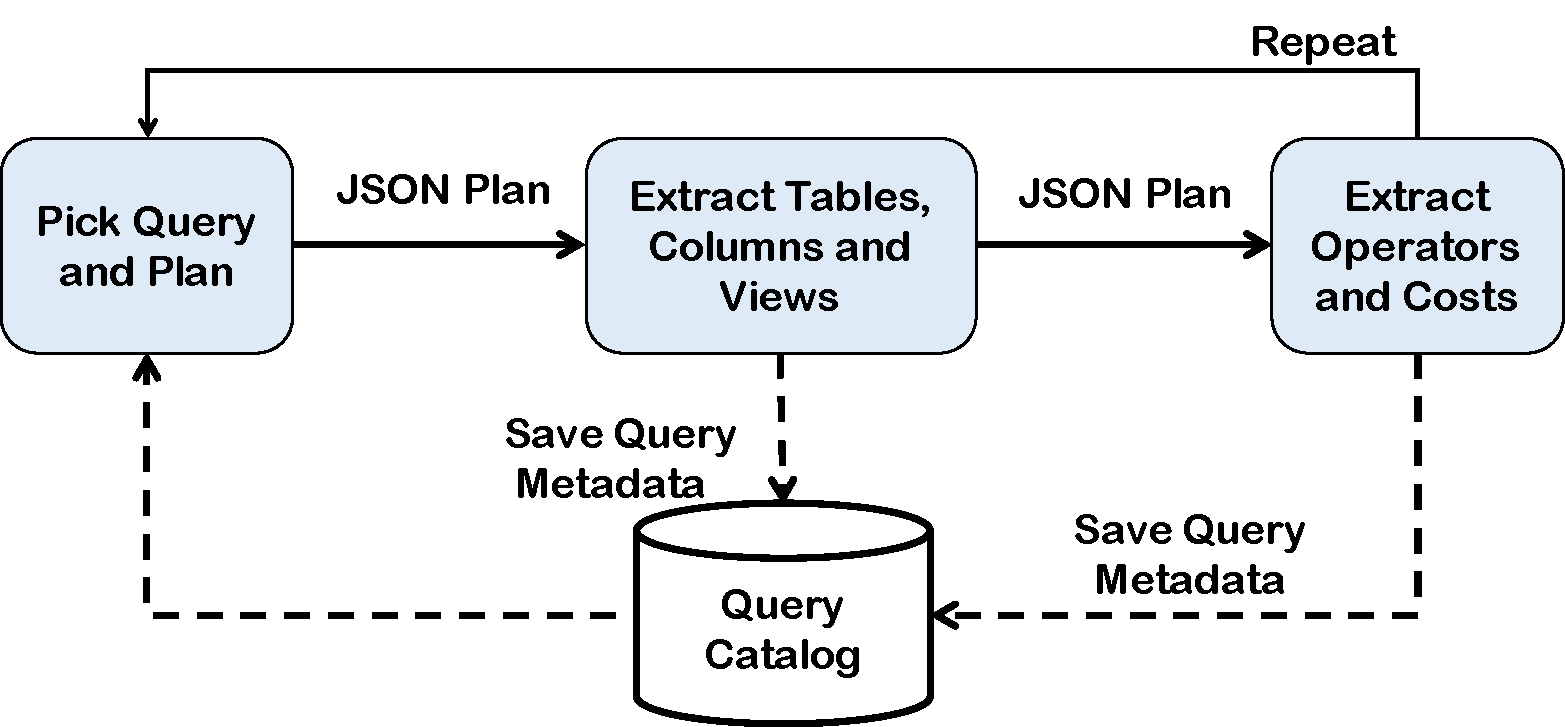
\includegraphics[width=.4\linewidth]{method_phase2.pdf}}
\caption{Workload Analysis Methodology}
\vspace{-15pt}
\end{figure*}

\lstref{lst:plan} shows a sample query and the corresponding extracted properties.
Most SQL providers support the `query explain' feature, which returns a raw query plan in the XML format, so the methodology explained in this section can be applied to other workloads as well. 
We implemented and bundled all functionality as a python library whose source code is available online on demand \footnote{\url{https://github.com/uwescience/query-workload-analysis}}.
As a sample implementation for other workloads, we have provided code to perform this analysis on SDSS and TPCH~\cite{council2008tpc}.
The python library also implements most of analysis that we make in the sections that follow.

\begin{listing}[h]
\begin{minted}{yaml}
  query: "SELECT * FROM incomes
             WHERE income > 500000"
  physicalOp: "Clustered Index Seek"
  io: 0.003125
  rowSize: 31
  cpu: 0.0001603
  numRows: 3
  filters:
    - "income GT 500000"
  operator: "Clustered Index Seek"
  total: 0.0032853
  children: []
  columns:
    incomes:
      - "name"
      - "income"
      - "position"
\end{minted}
\caption{Extracted structure and properties from a sample query.}
\label{lst:plan}
\end{listing}


The total size of the query logs along with this meta data (\eg JSON query plans) is $398$ MB. This will also be made available publicly.
A summary of metadata extracted from \sqlshare{} logs is shown in table \tabref{t:summarymetrics1} and \tabref{t:summarymetrics2}.
As mentioned in \secref{sec:datamodel}  \sqlshare{} creates trivial views over base tables to remove the distinction between a table and a view. 
Hence for analysis that follows in the later section, we will only look at the non-trivial views (\ie the ones explicitly created by users) unless otherwise specified.

\section{Evaluation of \SQLSHARE{}\\Features}
\label{sec:features}

In this section, we consider the specific features of \sqlshare{} and analyze their effect on the usage patterns we see in the workload.
Each subsection represents a key finding associated with a specific feature of \sqlshare{}.
\reviewmeta{We have conducted interviews with our most active users, who are primarily researchers in the life, earth, and social sciences.  Statements about our users' backgrounds and requirements are informed by these interviews.}

\subsection{Relaxed Schemas Afford Integration}
\label{sec:relaxedschema}

\reviewone{The requirement for relaxed schemas is motivated by the ubiquity of \emph{weakly structured} data. Further, the collaborative nature of data science results in a need to frequently share intermediate results before the data has been properly organized and described.  As a result, we designed \sqlshare{} to tolerate (and even embrace) upload of weakly structured data, encouraging users to write SQL queries to repair and reorganize their data.
We build evidence to support this hypothesis by searching the corpus of $4535$ derived datasets (views) for specific SQL idioms that correspond to ``schematization'' tasks: cleaning, typecasting, and integration.

\emph{NULL injection}: About $220$ of the derived datasets use a \texttt{CASE} expression to replace special values with NULL. ii) \emph{Post hoc Column Types}: After removing bad tuples and replacing missing values with NULL, we find that about $200$ of derived datasets used SQL \texttt{CAST} to introduce new types on existing columns. 

\emph{Vertical Recomposition}: Datasets presented to \sqlshare{} are often decomposed into multiple files that reflect the manner in which the data was collected.
Rather than requiring that these files be concatenated offline or requiring that a single table be designed to store all such data, we encourage users to ``upload first, ask questions later.''  We found evidence of about $100$ datasets that involved vertical recomposition using UNION in SQL.

\emph{Column Renaming}: Datasets presented to \sqlshare{} frequently had no column names in the source file; \sqlshare{} automatically assigns default columns names in these cases and we encourage users to write SQL to assign semantic names.  We see $1996$ uploaded tables (about 50\%) that had at least one default-assigned column name and $1691$ uploaded tables for which \emph{all} columns names were assigned a default value. Almost $16\%$ of datasets involve some kind of column renaming step, suggesting that users have adopted SQL as a tool for adding semantics to their data. Rejecting datasets due to incomplete column names would have clearly limited uptake.

Overall, the data suggests that relaxed schemas played an important role in many use cases, and that tolerance for weakly structured data is an important part of any data system targeting science and data science environments.}

\subsection{Views Afford Controlled Data Sharing}
\label{sec:datasets}
\reviewone{The view-centric data model of \sqlshare{} (\figref{fig:datamodel}) allows users to think in terms of logical datasets rather than 
understanding a distinction between physical tables and virtual views.  
The hierarchy of derived views provides a simple form of provenance; the user can inspect (and with permission, edit) the specific steps applied to produce the final result.
The view-centric data model also affords collaboration: users can share the derived dataset (and its provenance) without emailing files that get out of sync with the master data.  Moreover, collaborators can directly derive their own datasets in the same system, and the provenance relationship is maintained.
The view-centric data model was a very successful feature in \sqlshare{}: About $56\%$ of the datasets in the system are derived from other datasets using views. Among the top 100 most active users, multi-layer view hierarchies were quite common.  \figref{fig:viewdepth} shows the max depth of dataset hierarchies forthese 100 users.  A view that references only base datasets is assigned a depth of 0. 
Other users would use views as query templates: They would use apply the same query to multiple source datasets, copying and pasting the view definition and only changing the name of a table in the FROM clause.
Copy-and-paste seems inadequate here; motivated by this finding we intend to lift parameterized query macros into the interface as a convenience function\footnote{A query macro would be different than a conventional parameterized query, since it allows parameters in the \texttt{FROM} clause rather than only as expressions.}.}
\begin{figure}[h]
\includegraphics[width=\linewidth]{plot_query_viewdepth.eps}
\caption{The maximum view depth for the 100 most active users of \sqlshare{}. The data suggest that the ability to derive and save new datasets using views was an important features.}
\label{fig:viewdepth}
\end{figure}

\reviewone{The view-centric data model also facilitates sharing: users can set daatset-level permissions, which are implemented in the database as view permissions.
A dataset can either be private, public or shared with specific set of users. 
The permissions features were heavily used.  About $37\%$ of the datasets in \sqlshare{} are publicly accessible, even though the default is to keep data private. About $9\%$ of the datasets were shared with a specific other user.  Moreover, about $2.5\%$ of the views access other datasets that the author does not own, and over $10\%$ of the queries logged in the system access datasets that the query author does not own. 
Beyond just collaborative analysis, the permissions feature allowed \sqlshare{} to function as a data publishing platform. Several users cited \sqlshare{} datasets in papers.  One user minted DOIs for datasets in \sqlshare{}; we are adding DOI minting into the interface as a feature in the next release.}

\subsection{Frequent SQL Idioms}
\label{sec:fullsql}
\reviewmeta{\sqlshare{} was designed to facilitate access to full, standards-compliant SQL as opposed to relying on the simplified SQL dialects often associated with analytics and sharing platforms (e.g., HIVE SQL~\cite{hivesql}, Google Fusion Tables~\cite{gonzalez2010google}). 

To evaluate whether full SQL was actually warranted, we counted the queries that use specific SQL language features that are sometimes omitted in simpler SQL dialects.  As one might expect, queries involving sorting were comon (24\%), and top k and outer join queries were frequent enough to justify support in any system (2\% and 11\% respectively).  Perhaps more surprisingly, window functions (expressed using the SQL-standard OVER clause) appeared in about 4\% of the workload. Virtually no systems outside of the major vendors support window functions; these newer systems will not be capable of handling the \sqlshare{} workload!

In addition to specific SQL language features, we found evidence of recurring SQL ``idioms'' or ``design patterns'' that might motivate higher-level convenience functions to support query authoring.  Aggregating timeseries and other data by computing a histogram was common enough (and awkward enough) that we are considering adding special support.  Another common but tedious pattern was to rename a single column, and then be forced to explicitly list out every other column in the table.  An expanded regular expression syntax raning over column names beyond just \texttt{*} is warranted: the ability to refer to all columns except a given column, or to replace a single column in its original order would be useful. More generally, the ability to refer to and transform a set of related columns in the same way would simplify query authoring: The expression \texttt{SELECT CAST(var* AS float) as \$v FROM data} could indicate ``replace each column with a prefix of \texttt{var} with an expression that casts it as a number and renames the expression appropriately.''}

\section{Workload Analysis}
\label{sec:workload}

In contrast to the conventional relational use cases characterized by a pre-engineered schema and predictable query patterns generated by the constraints of a client application, we hypothesized that \sqlshare{} users would write queries that are more complex individually and more diverse as a set, making the corpus more useful for designing new systems.
A more complex workload, especially one derived from hand-written queries, provides a more realistic basis for experiments in optimization, query debugging, and language features than a workload from a conventional, sanitized environment.

To test this hypothesis, we need to define metrics for query complexity and workload diversity. \reviewone{Since we are onboarding users with little or no database experience, query complexity needs to be measured in terms of the `cognitive' effort it takes to express a task as a SQL query. Thus, the measures like query runtime or latency alone do not show the correct picture. In the discussion that follows, we have attempted to find proxy metrics to capture this `cognitive' complexity.} We develop simple metrics in this section and show that \sqlshare{} queries on average tend to be more complex and more diverse than those of a conventional database workload generated from a comparable science domain: the Sloan Digital Sky Survey (SDSS)~\cite{kent1994sloan}.

The SkyServer project of the SDSS is a redshift and infrared spectroscopy survey of galaxies, quasars, and stars.
It led to the most detailed three-dimensional map of the universe ever created at the time.
The survey consists of multiple data releases (10 to date), which represent different projects and different stages of processing
refinement. Besides the survey data, the SDSS database contains one of the few publicly available query workloads from a live SQL database supporting both ad hoc
hand-authored queries as well as queries generated from a point-and-click GUI. Singh \ea, in the Traffic Report for SDSS~\cite{singh2007skyserver} describe how during the first five years itself the system generated $180GB$ of logs. These logs were then normalized and cleaned and auxiliary data structures were built for analysis.
SDSS is a useful comparison: it is a conventional database application with a pre-engineered schema but the users and tasks are not dissimilar to those of \sqlshare{}.

\subsection{\sqlshare{} Queries are Complex}

We interpret query complexity primarily as a measure of the cognitive load on the user during query authoring as opposed to computational compelxity in optimizing or evaluating the query.  Our goal is to design lightweight data systems that can be used as part of day-to-day analytics tasks, which means we are competing directly with general purpose scripting languages for users' attention.  Any query corpus that purports to reflect the usage patterns of analysts cannot rely on vanilla query patterns typically assumed in the database literature. 
In this section, we consider ASCII character length as a simple proxy for query complexity and then argue why the number of distinct operators is an improvement.


\paragraph*{ASCII Query Length}

A naive estimate of query complexity from both the user and system perspective is the character length of the query as a string.  The premise for character length as an indicator of complexity is is that the longer the query, the more a user has to write and read, and the more time and effort it takes to craft the query.

In both \sqlshare{} and SDSS, most queries are short.  But a significant number of queries in \sqlshare{}, about $1500$, are greater than $500$ characters. This is not surprising given that users write queries over datasets which are often decomposed into multiple tables.  \figref{fig:qlengthcdf} shows the histogram of query length for both \sqlshare{} and SDSS. 
SDSS has a high percentage of queries with similar length. We investigated this further and found that there are clear categories of SDSS queries corresponding to specific lengths. These categories correspond to particular query templates and example queries used many times, demonstrating that few of these queries should be considered hand-written.
In addition, the shortest 20\% of both workloads are less than 100 characters, which is quite short.  But the longer queries in \sqlshare{} range upto $11375$ characters. 
However, query length does not necessarily capture cognitive complexity since long queries may involve repetitive patterns that are easy to write via copy-and-paste.  
We see examples of queries that are over 1000 characters long but involve just two operators (a filter applied to 50+ columns).
The takeaway from the length comparison however is that \sqlshare{} users write queries that the database community would consider unusual, which is precisely why this corpus is valuable.  Such queries should be considered in any realistic workload targeting weakly structured data and non-expert users.

\begin{figure}
\centering
\includegraphics[width=.9\columnwidth]{plot_length_cdf.eps}
\caption{Hand-written \sqlshare{} queries tend to vary more widely in length than SDSS queries.  Short queries tend to be shorter, but long queries tend to be longer.  SDSS queries show evidence of being ``canned'' rather than hand-written: only a few distinctive lengths are present and the majority of SDSS queries are about 200 characters.  We explore these patterns in more detail in \secref{sec:entropy}.}
\label{fig:qlengthcdf}
\end{figure}

\paragraph*{Distinct Operators in Query}

To capture the complexity of a query more accurately, we look at the number of operations in the execution plan.
More operations mean more steps of computation which increases the complexity of scheduling of data flow for the system. 
\sqlshare{} queries use a lot more operators than SDSS on an average.
Many operations alone does not necessarily lead to a complex query for a user if the query uses the same operator over and over \eg a union of 10 relations.
A better metric to capture this case is to look at the \emph{diversity} of operators and count the number of unique operators per query.
A combination of both the number of operations and the number of distinct operations intuitively captures complexity better than either of the two metric.
\begin{figure}[h]
\centering
\vspace{-1pt}
\includegraphics[width=.9\columnwidth]{plot_num_dist_physops_cdf.eps}
\caption{CDF of the number of distinct operators per query in both workloads. \sqlshare{} has many queries with very few distinct operators, but about $5-8\%$ of the most complex queries have many more distinct operators than SDSS, \reviewthree{suggesting that most complex queries in \sqlshare{} appear to be more complex than the most complex queries in SDSS.}}
\label{fig:distopscdf}
\vspace{-8pt}
\end{figure}
\figref{fig:distopscdf} shows the number of distinct operators for the three workloads. 

While a majority of queries in the \sqlshare{} workload consist of $<4$ distinct operators, a significant percentage of queries have significantly higher number of distinct operators, suggesting higher complexity.  Among the top 10\% of the queries with the highest number of distinct operators, the \sqlshare{} queries tend to have almost double.

The next question one might ask is what type of the operators are present in the workload as a whole.
This metric helps us understand workload complexity by providing the minimum requirement of SQL features for the workload to run, which is of interest to system designers.

\begin{figure}[h]
\centering
\includegraphics[width=\columnwidth]{plot_ops_sqlshare.eps}
\vspace{-12pt}
\caption{The most commonly used physical operators in \sqlshare{}. We ignored Clustered Indexed Scan because \sqlshare{} uses SQLAzure which requires them. Presence of a lot of aggregate and arithmetic operators in \sqlshare{} suggests the presence of analytic workloads.}
\vspace{-9pt}
\label{fig:pOpssqlshare}
\end{figure}
\begin{figure}[h]
\centering
\includegraphics[width=\columnwidth]{plot_ops_sdss.eps}
\vspace{-14pt}
\caption{The most-used operator in SDSS is computation on scalars as a lot of queries use UDFs. Compared to \sqlshare{} we see fewer arithmetic and aggregate operators.}
\vspace{-12pt}
\label{fig:pOpsSDSS}
\end{figure}
\figref{fig:pOpssqlshare} and \figref{fig:pOpsSDSS} show the ten most common operators in \sqlshare{} and SDSS.
We ignored `clustered index scan' for \sqlshare{} workload because \sqlshare{} uses SQLAzure as its backend and SQLAzure requires that every table be associated with a clustered index.
\sqlshare{} is dominated by aggregate queries, while SDSS has mostly computations on scalars most likely because it consists of a lot of user defined functions\footnote{\url{http://skyserver.sdss.org/dr5/sp/help/browser/shortdescr.asp?n=Functions&t=F}}.
Overall, we find indications that users write more complex queries in \sqlshare{}, suggesting that support for full SQL is useful for users.

\subsection{\sqlshare{} Queries are Diverse}
\label{sec:sqlsharediverse}
If users are writing ad hoc queries rather than operating an application that generates queries on their behalf, we would expect that the \emph{diversity} of the workload to increase. Rather than having the entire workload reduced to a few repeating templates, each query would be more likely to be unique. 
As the diversity of a query workload increases, system design and performance management becomes more challenging: up-front engineering and physical tuning becomes less efficacious.  We consider high diversity a characteristic feature of the data science workloads and an important design goal of any system targeting this domain. 
This makes diversity an important feature to consider in database research. Current system overspecializes in simpler queries, since a corpus of hand-written real queries is unavailable. For example, research on query recommendation platform like SnipSuggest~\cite{snipsuggest} can be further improved by taking real science queries into consideration to reflect the full complexity of the problem. 
Similarly, query optimizers should consider optimizations for arithmetic optimizations as well. New languages or user interfaces which make common science idioms simpler would greatly increase scientists' productivity.

We can consider the question of whether \sqlshare{} workloads are measurably more diverse than the workloads
of a conventional database application such as SDSS.

\paragraph*{Workload Entropy}
\label{sec:entropy}
\reviewone{To quantify workload entropy, we must define query equivalence.  
A simple but na\"{i}ve metric is exact ASCII string equivalence.
ASCII string equivalence can only help eliminate very simple kinds of redundancies, such as identical queries generated by applications or repeated instances of copy-and-pasted sample queries. The SDSS workload contains both of these patterns, however, so we included this definition in our analysis.

A better measure of query equivalence was proposed by Mozafari \ea \cite{mozafari2015cliffguard}: A query is represented by the set of all attributes (columns) referenced by the query. If two queries reference different sets of attributes, we say they are \emph{column distinct}. A weakness of this metric in our context is that the set of attributes referenced does not capture the user's intended task, and can therefore fail to distinguish queries that differ widely in layers of nesting, use of complex expressions (e.g., theta joins or window functions), and grouping structures.
The presence or absence of these features may be what determines whether a query is perceived as ``difficult'' to novice users, which is an important consideration in the design of a system.

ASCII string equivalence overlooks equivalences and the column-based metric proposed by Mozafari \ea appears to overlook differences.  We therefore propose a simple third metric by extracting a query plan and normalizing it by removing all constants. 
We obtain an optimized query plan from the database, which also contains estimated result sizes and estimated runtimes for each operator. The query plan resolves any heterogeneity resulting from the syntax (order of conditions, JOIN vs. WHERE, nesting vs. joins, etc.) 
In addition, we remove all constants and literals from the plan to create the \emph{query plan template} (QPT). 
The QPT seems to offer a better description of the user's intended task, as it unifies most semantically equivalent
queries but still incorporates the operations.


The SDSS workload initially contained $7M$ queries. 
However, after resolving redundant queries using simple string equivalence, the SDSS workload contained only about $200K$; $3\%$ of the total.
Many queries in the SDSS are actually not handwritten; they were generated by applications such as the Google Earth plugin or the query composer from the SkyServer website
.
In contrast, the \sqlshare{} workload from 2011 to 2015 contains about $25K$ queries, $24096$ ($96\%$) of which were unique.

If we group queries by the set of columns referenced following Mozafari \ea, we find that $45.35\%$ of the queries are distinct in the \sqlshare{} workload compared with only $0.2\%$ of the 200K string distinct queries for SDSS.}

\begin{table}[h]
\centering
\begin{tabular}{| p{2.4cm} | p{2.4cm} | p{2.4cm} |}
\hline
Diversity Metric & SDSS & \sqlshare{} \\ \hline
Total queries & $7M$ & $25052$ \\ \hline
String distinct queries & $200K$, $3\%$ of $7M$ & $24096$, $96\%$ of $25052$ \\ \hline
Column distinct queries & $467$, $0.2\%$ of $200K$ & $10928$, $45.35\%$ of $24096$\\ \hline
Distinct query templates & $686$, $0.3\%$ of $200K$ & $15199$, $63.07\%$ of $24096$ \\ \hline
\end{tabular}
\vspace{-10pt}
\caption{\reviewone{Workload Entropy: \sqlshare{} queries are more diverse and have $63\%$ distinct query templates. For SDSS, the number is very low ($0.3\%$).}}
\label{t:entropy}
\end{table}

\reviewone{Finally, SDSS only exhibits $686$ unique query plan templates ($0.3\%$ of the $200K$ string distinct queries).
The low entropy is not unexpected, given that many users manipulate a GUI and use standard examples queries to study a fixed schema. 
The \sqlshare{} workload contains significantly higher entropy:
It has about $15199$ ($63.07\%$ of the $24096$ string distinct queries) unique query plan templates. 
We summarize these findings in \tabref{t:entropy}. While none of these measures are perfect, a high value of ($\frac{\rm Unique\;Queries}{\rm Total\;Queries}$) and a high absolute number of unique queries indicate high diversity in a workload, suggesting that the \sqlshare{} workload is an appropriate test case to drive requirements of new systems.
 
We see two distinct usage patterns here in the two database-as-a-service platforms, \sqlshare{} and SDSS. Since SDSS relies on a fixed, engineered schema, the diversity of queries they can ask is obviously limited.
\sqlshare{} allows users to upload arbitrary tables; there is no expectation that queries will overlap in form or content. 
}
\paragraph*{Expression Distribution}

\label{sec:types_exprs}
Another measure of query diversity is the type and distribution of expression operators.
We found the number of different expression operators to be $89$ for \sqlshare{} and $49$ for SDSS.
Moreover, we found that the workloads with intuitively higher variety not only use more diverse expressions but also more user defined functions (UDFs):
\sqlshare{} has $56$ and SDSS $22$.
The most common intrinsic \footnote{\url{https://technet.microsoft.com/en-us/library/ms191298(v=sql.105).aspx}} and arithmetic expressions in SDSS are two scalar expressions followed by \texttt{BIT\_AND}, \texttt{like} and \texttt{upper} (\tabref{table:sdss_ops}).
In \sqlshare{} we found that six out of the ten most common expression operators (and again the vast majority) are operations on strings: \texttt{like}, \texttt{patindex}, \texttt{isnumeric}, \texttt{substring}, \texttt{charindex}, and \texttt{len} (\tabref{table:sqlshare_ops}).
Also, \sqlshare{} has a higher expression diversity than other 2 workloads.
This expression diversity backs our original hypothesis that use cases for \sqlshare{} go beyond just data management and also include \emph{data ingest, integration and cleaning} as suggested by the prevalence of string operations.
\begin{table}[h]
\begin{subtable}{0.45\columnwidth}
  \centering
    \begin{tabular}{| l | l |}
  \hline
  Operator  & Count \\ \hline
  like      & 61755 \\ \hline
  ADD     & 31570 \\ \hline
  DIV     & 17198 \\ \hline
  SUB       &  13707 \\ \hline
  patindex  &   8212 \\ \hline
  substring &   7490 \\ \hline
  isnumeric &   7206 \\ \hline
  charindex &   6364 \\ \hline
  MULT      &  4162 \\ \hline
  square    &   2636 \\ \hline
  len       &   2608 \\ \hline
  \end{tabular}
  \caption{\sqlshare{}}
  \label{table:sqlshare_ops}
\end{subtable}
\begin{subtable}{0.45\columnwidth}
  \centering
    \begin{tabular}{| p{2.5cm} | l |}
  \hline
  Operator  & Count \\ \hline
  GetRange\newline ThroughConvert      &  25746 \\ \hline
  GetRangeWith\newline MismatchedTypes &  25746 \\ \hline
  BIT\_AND                     &  21850 \\ \hline
  like                        &   2376 \\ \hline
  upper                       &   2312 \\ \hline
  \end{tabular}
  \caption{SDSS}
  \label{table:sdss_ops}
\end{subtable}
\vspace{-10pt}
\caption{Most common intrinsic \& arithmetic expression operators. String operations are very common on \sqlshare{}, suggesting a lot of data integration and munging tasks.}
\vspace{-12pt}
\end{table}

\paragraph*{Reuse: Compress Runtimes}
\label{sec:reuse}
The overall runtime of query is a measure of its complexity, but its misleading because runtime gets affected by the data size as well. 
However, runtime that can be saved by identifying re-occurring clauses in queries is a good measure of query diversity, \ie lower reuse potential suggests higher diversity.
Roy \ea show experiments in which $30\%$ to $80\%$ (depending on the workload) of the execution time can be saved by aggressively caching intermediate results~\cite{roy2000don}.
Query optimization in the presence of cached results and materialized views is beyond the scope of this paper.
Nonetheless, we implemented a simple algorithm to calculate reuse of query results that matches subtrees of query execution plans.
While iterating over the queries, all subtrees are matched against all subtrees from previous queries.
We allow a subtree that we match against to have less selective filters (filters are a subset) and more columns for the same tables (columns is a superset).
If we find that we have seen the same subtree before, we add the cost of the subtree as estimated by the SQLServer optimizer to the saved runtime.
Consequently, a precomputed intermediate result does not cost us anything when being reused.

Although this algorithm does not accurately model the actual execution time, we use it to estimate how diverse queries are.
The algorithm can underestimate the potential for reuse since the matching misses cases when a rewriting would be needed.
It could overestimate since we assume infinite memory as well as no cost for using a previously computed result.
In this analysis we removed duplicate queries since a query that appears again will completely reuse previous results (recall that over $90\%$ of SDSS queries are duplicates. But even for the distinct queries, $14\%$ of the runtime could be saved.
In SQLShare, we estimate saving to be around $37\%$.
In all workloads, most of the saving per query was either very high (more than $90\%$) or very low (less than $10\%$).
We conclude that most of the reuse could be achieved with a small cache if we have a good heuristic to determine which results will be reused. This also confirms our hypothesis that \sqlshare{} queries are indeed more diverse.


\subsection{Dataset Permanence Varies by User}

In a conventional RDBMS, the schema is not expected to change much over time.
We calculated the lifetime for the datasets in \sqlshare{}, with lifetime defined as the difference in days between the first and the last time that dataset was accessed in a query and found that the \sqlshare{} workload exhibits a variety of patterns.  In particular, many users are operating in short-duration analysis loops, where they upload some data, write a few queries, and then move on to another task.  
This usage pattern is atypical for relational databases and seems to motivate new system features, including some of those already implemented in \sqlshare{}.

\figref{fig:shortlifetime} shows the lifetime in days for the datasets for a user who both continuously updated new datasets and frequently accessed previous datasets.  Each point represents one dataset for the given user.  The y-axis is the number of days between the first and last query that accessed the dataset. While many datasets are used across periods of years, the majority are uploaded once, analyzed over a period of 5-7 days, and never accessed again.  For this user, over half are only accessed once, on the same day they are uploaded. 
\begin{figure}[h]
\centering
\includegraphics[width=.9\columnwidth]{plot_query_lifetime.eps}
\vspace{-10pt}
\caption{Dataset lifetimes for 12 most active users in \sqlshare{}. Each curve is a user. The y-axis is the number of days between the first and last time the dataset was accessed. The x-axis is rank order. The great majority of datasets are accessed across a span of less 10 days, but some are accessed across periods of years. This type of a workload, where a user explores the data and never accesses it again, is a departure from a conventional RDBMS use case. The highlighted user is the most active user in \sqlshare{}.}
\label{fig:shortlifetime}
\vspace{-10pt}
\end{figure}
%We find that some users have most datasets with life less than 5-7 days, and a handful have life spanning to hundreds of days.
Some users operate exclusively in a ``data processing'' mode, where they upload data at a predictable rate, process it using the same queries, and move on.
The shorter dataset lifetimes associated with science and data science workloads is significant because it suggests that the costs associated with creating schemas and loading data would be incurred so frequently as to make these workloads infeasible (or at least unattractive) for conventional database systems.  
This limitation does not exist in \sqlshare{} due to the simple schema inference mechanisms and the web-hosted delivery vehicle.

\sqlshare{} users in general are varied in their patterns of data upload and data analysis.
\figref{fig:tablecoveragetopusers} shows table coverage for the most active users in \sqlshare{}. Table coverage measures the cumulative count of tables referenced by queries upto a certain point in time. The figure shows how new datasets are being added all the time.
This suggests that the use case is the following: user keeps adding datasets, and the queries are usually written on \emph{all} of the datasets taken together, and that she may be uploading data to overwrite/replace old tables then re-running the same queries.

\begin{figure}[h]
\includegraphics[width=.9\columnwidth]{plot_table_coverage.eps}
\vspace{-10pt}
\caption{The rate of table coverage over time for the 12 most active users. 
Highlighted in red is the most active user for \sqlshare{}. 
Each curve corresponds to a user and describes the percentage of tables accessed by the first N\% of queries. A user who uploads one table at a time and queries it once would generate a line of slope one. Curves above slope one indicate a more conventional workload, where the user uploads many tables and then queries them repeatedly.  Curves near to or below slope one indicate a more ad hoc workload, where queries are intermingled with new dataset uploads. We see both usage patterns in \sqlshare{}, but the ad hoc pattern dominates.}
\label{fig:tablecoveragetopusers}
\vspace{-10pt}
\end{figure}

\subsection{\sqlshare{} Attracts High-Churn Work}
\reviewone{Based on interviews with users, \sqlshare{} seemed to be used to support workloads that exhibited higher ``churn'' than conventional databases, where datasets would be uploaded, queried a few times, and then put aside.  
To attempt to quantify our anecdotal evidence, we considered the ratio of queries to datasets for each user, hypothesizing that this ratio would be very low for most \sqlshare{} users.

\figref{fig:qd} shows the results. Each point is a single user.
The x-axis is the number of distinct datasets owned by that user and the y-axis is the 
number of distinct queries submitted by that user.  Both axes are on a log scale.
The variety in workloads is also apparent: a few users upload relatively few tables (10-30) and query them repeatedly,
which is reminiscent of a conventional database workload.  These queries are labeled \textsf{Analytical} in the plot.
But most users tend to upload approximately the same number of datasets as the number of queries they write, suggesting an ad hoc, exploratory workload.  These users are labeled \textsf{Exploratory}.  We also see that some users uploaded exactly one dataset, wrote 1-50 queries, and then never return.  This group surely includes some users who were simply trying out the system and who either never had an intention to use it or did not find it useful.  We label this group \textsf{One-shot users}.

To quantify the notion of workload diversity, we adapt the methodology of Mozafari et al \cite{mozafari2015cliffguard}: break each user's workload into chronological blocks and measure the distance between the chunks. Each chunk is considered a separate workload and is represented by a row vector. Each position in this vector corresponds to a unique subset of attributes from the database. The value at that position represents the normalized frequency of queries that reference exactly this set of attributes. We then calculate the \emph{euclidean} distance between these vectors, following Mozafari's algorithm \cite{mozafari2015cliffguard}. The maximum distance found in the original paper was $0.003$; this number was considered a high workload diversity. Among those users with sufficient queries to support this analysis, many exhibited \emph{orders of magnitude} more diversity in their workload.}

\begin{figure}[h]
\centering
\includegraphics[width=.9\columnwidth]{plot_Q_D.eps}
\vspace{-10pt}
\caption{The ratio of datasets to queries suggests different usage patterns. The y-axis is the log of the number of queries, and the x-axis is the log of the number of datasets. Each point represents one user.  Exploratory users only write a small number of queries over each dataset they upload. Some users exhibit a more conventional usage pattern, uploading a relatively small number of datasets and querying them repeatedly. A few non-active users upload one table and write very few queries.}
\label{fig:qd}
\vspace{-5pt}
\end{figure}

\section{Related Work}
\label{sec:relatedwork}

Structure extraction tools cast the data variety problem as one of parsing complex formats to produce (weakly) structured data for further processing. OpenRefine~\cite{refine} and Wrangler~\cite{kandel2011wrangler} are examples of this approach. These tools offer no support for working with multiple datasets or managing complexity once the parsing step has been completed, which has been shown to be a dominant cost~\cite{analysis-interviews}. 
In traditional data integration approaches the central goal is to derive a mediated schema from two or more source schemas, allowing all source data to be queried uniformly~\cite{doan2005semantic}.
Tools and algorithms in this area induce relationships between database elements (tables, columns, rows) and use these relationships to rewrite queries or restructure data. Despite a long history of research (and a detour through XML in the early part of this century), these techniques do not seem to be widely used by analysts today, in part because of the assumptions that the input schemas are carefully engineered, information carrying structures on which the algorithms can gain purchase. 

A welcome departure from the engineered schemas assumed by data integration techniques was \emph{dataspaces}~\cite{franklin2005databases}.The paper was prescient in its ability to capture important aspects of the high variety problem, but focused heavily on enterprise settings and managed environments rather than the ad hoc, one-off analysis that characterizes data science activities we see in practice. It is unusual to assume that we would know all kind of operations and all sources of data before hand. This approach misses the point that in Big Data, data sources and the operations required are usually not known beforehand. 
However, in case of \sqlshare{}, the departure from the above mentioned approaches is that it
enables scientific data analysis with a bare minimum set of changes to the original RDBMS.
Infact, at its core, \sqlshare{} uses pure relational models. It just hides these from the users.
Our work shows that how even with these basic changes, we can cater to the entire data lifecycle, \ie ingest, cleaning, synthesis, management, analytics, visualization and sharing. 

Khoussainova \ea noted in~\cite{khoussainova2009case} that the mode of interaction with databases is changing. Data analytics warrants the support for exploratory queries, query recommendations and collaborative query management. We believe \sqlshare{} is a right step in this direction.
Bhardwaj \ea presented DataHub~\cite{bhardwaj2014datahub}, a system which provides the collaborative data management and versioning, but unlike \sqlshare{} it lacks data querying capabilities and support for full SQL.

SnipSuggest~\cite{snipsuggest} is an example of a system which can enable non-experts to write complex SQL queries and even teach them. 
This work is complementary to one aspect of \sqlshare{} \ie reducing `friction' for query authoring.
It would be interesting to see how user query complexity changes overtime using SnipSuggest with \sqlshare{}.
Ogasawara \ea~\cite{ogasawara2011algebraic} presented support for automatic optimization data science workflows, motivating research in database support for scientific workloads.
Recently, Fei \ea presented Schema-Free SQL~\cite{schemafreesql} which tries to enables faster analysis of data for which the schema is unknown. This approach is different from the automatic schema inference in \sqlshare{} and builds language support for inaccurate/unknown schema.

Ren \ea performed a workload analysis over $3$ different Hadoop~\cite{hadoop} research clusters~\cite{hadoopadolescence}. They noted underuse Hadoop features and significant diversity in workloads application styles motivating newer tools.
Singh \ea published a 5 year usage study of SDSS~\cite{singh2007skyserver} and reasoned about why it was so successful. Their work
analyzed traffic and sessions by duration, usage pattern over time and found interesting factors like
site's popularity and benefits of providing a framework for ad hoc SQL. 

\sqlshare{} takes this a step further by providing an SDSS like system for everyone. 
By enabling the user to upload datasets and enable sharing and dataset hierarchy, \sqlshare{}
unfolds a lot more avenues for easy scientific data management.

\section{Conclusion}
\label{sec:conclusion}
We presented a new public query workload corpus for use by the database research community and described the open source SQL-as-a-Service system \sqlshare{} that was deployed to collect it.  Further, we showed that the features of \sqlshare{} were instrumental in attracting new kinds of ad hoc queries that are written to perform tasks usually reserved for scripts and files.  Finally, we gave a preliminary analysis of the workload and argued that it is demonstrably more diverse than a comparable public workload in science, and that users are writing very complex queries by hand.

The \sqlshare{} system was designed to be  minimal adaptation of existing database technology to attract users in ad hoc, high-touch analytics environments.  We relaxed assumptions about schemas, inferring structure automatically from the data and tolerating various structural problems (mismatched row lengths, non-homogeneous types, missing column names).  We adopt a view-oriented data model to encourage reuse, track provenance, simplify editing, and facilitate data sharing. We support full SQL, finding that impoverised SQL-like languages are not sufficient to express the queries in our workload.  
We found these features of \sqlshare{} to be demonstrably useful by analyzing patterns in the workload.  More generally, we conclude that \sqlshare{} is useful for short lifetime, one-shot analysis tasks that are typically ill-suited for databases, and that these tasks produced queries that are more complex and more diverse.

To define query complexity, we considered character length of the query as an ASCII string and the number of distinct operators.  We showed that by these measures \sqlshare{} had attracted hand-written queries that are more complex than the most complex queries in the comparable Sloan Digital Sky Survey workload, another public query workload associated with a conventional database application in a comparable domain.

To define workload diversity, we considered the entropy of the workload: the number of unique queries divided by the number of total queries.  To define query uniqueness, we considered string uniqueness as a naive baseline, but recognizing that two queries that have an identical structure but differ in literal values should not be considered truly distinct.  We therefore considered a templatization procedure that unified the structure of queries in the log and created equivalence classes based on query patterns.  By both measures of entropy, the \sqlshare{} workload was more diverse than the SDSS workload.  We also considered the use of expressions and scalar functions.  While expressions were more varied in the \sqlshare{} dataset, the SDSS workload involved a significant number of user-defined functions.


In future work, we plan to use this workload to provide a formal definition for query complexity and design languages and editors that can provably reduce complexity.
We can use this definition to build more effective query recommendation engines which recommends queries of comparable complexity to queries that user has written before. 
We also plan to use the complexity and diversity properties of the query workload to design a formal benchmark emphasizing high variety rather than hig volume or high velocity.
Our analysis will also inform the development of new systems such as Myria~\cite{halperin2014demonstration} that are designed to address analytics workloads in science and data science.


\section{Acknowledgements}

This project was supported by NSF IIS award \# $1247469$, the Intel Science and Technology Center for Big Data
and the University of Washington eScience Institute, which made this work possible.

\newpage
\bibliographystyle{abbrv}
\bibliography{paper}
\end{document}
